\subsection{Threat Hunting}
Threat hunting is a forward-looking security strategy that involves scrutinizing data from logs, network traffic, and endpoints to find and mitigate cyber threats bypassing conventional security measures. Its goal is to identify latent threats within an IT environment. The method encompasses hypothesis creation, data gathering, analysis, and reaction.

Wazuh bolsters security teams in their threat hunting efforts, enabling swift actions to confine the threat and prevent further harm.

\subsubsection{Log Data Analysis}
This feature is elaborated later in \ref{log-data-analysis}. But to summarize, for a robust threat hunting approach, efficient log data collection and analysis are critical. Wazuh, as a comprehensive XDR and SIEM platform, facilitates \textbf{centralized log data collection}, integrating data from varied sources like endpoints, network devices, and applications for simplified analysis and enhanced monitoring efficiency.

Below is a depiction of the Wazuh dashboard settings for auditing log collection from a monitored endpoint.

\begin{figure}[H]
    \centering
    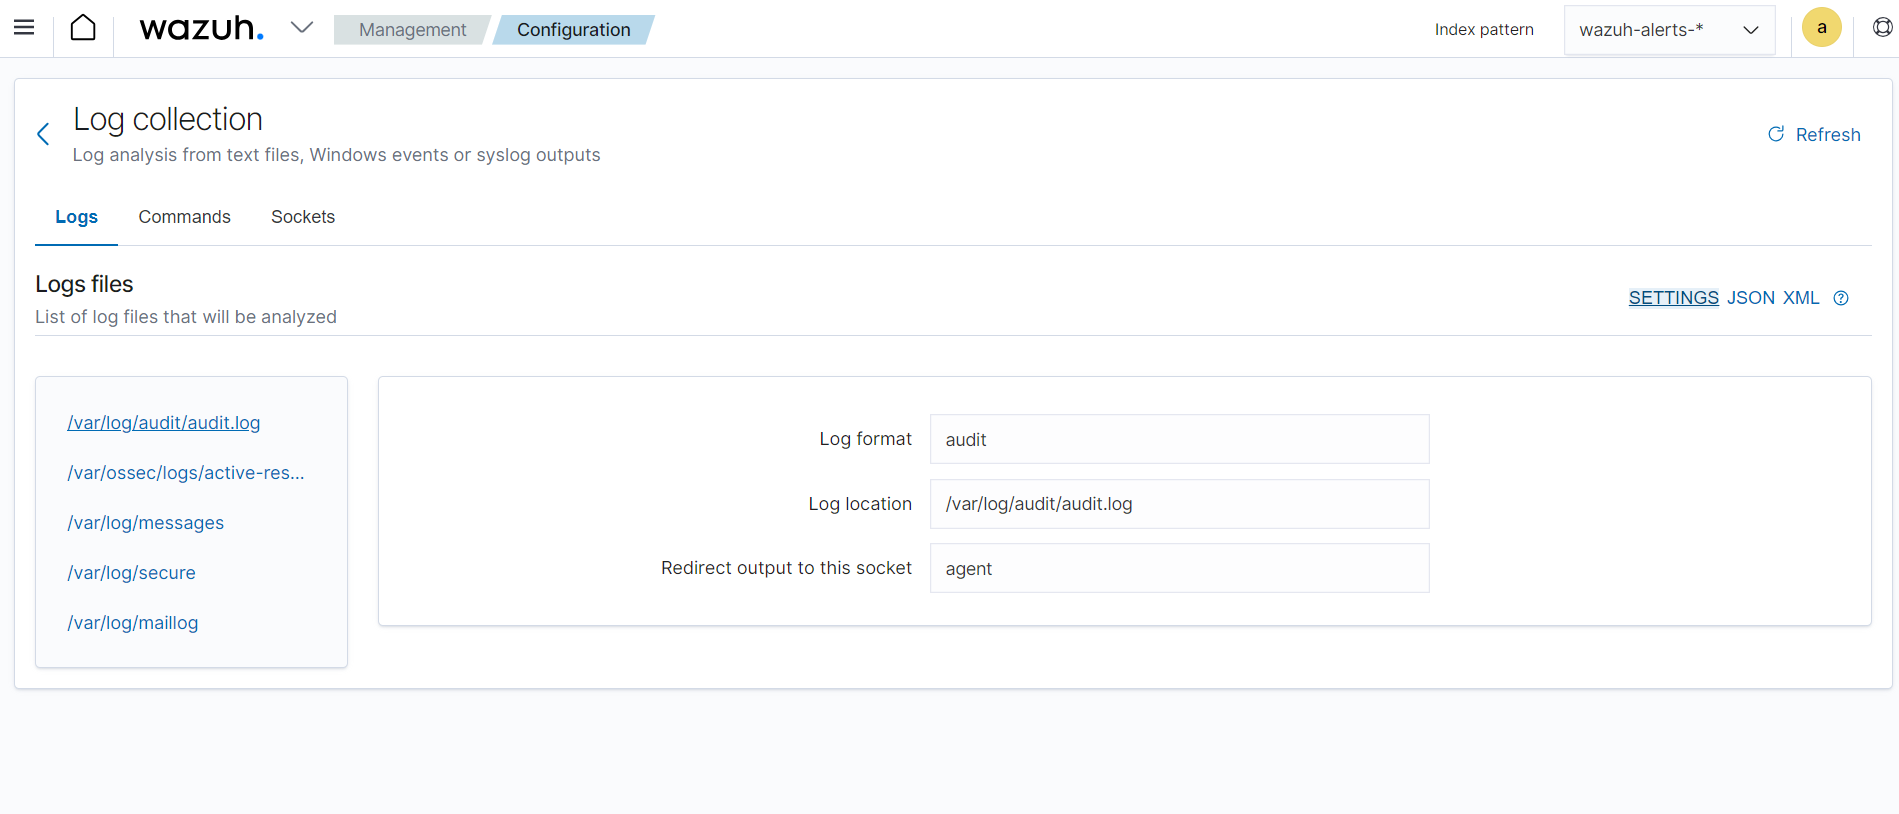
\includegraphics[width=0.8\textwidth]{images/threat-hunting/log-collection-settings.png}
    \caption{Log collection settings on the Wazuh dashboard}
    \label{fig:log-collection-settings}
\end{figure}

Wazuh employs decoders to parse valuable data from collected log files, breaking down raw data into discernible attributes like timestamps, IP addresses, and event types. The dashboard showcases the \texttt{wazuh-alerts-*} index pattern and its fields as seen below.

\begin{figure}[H]
    \centering
    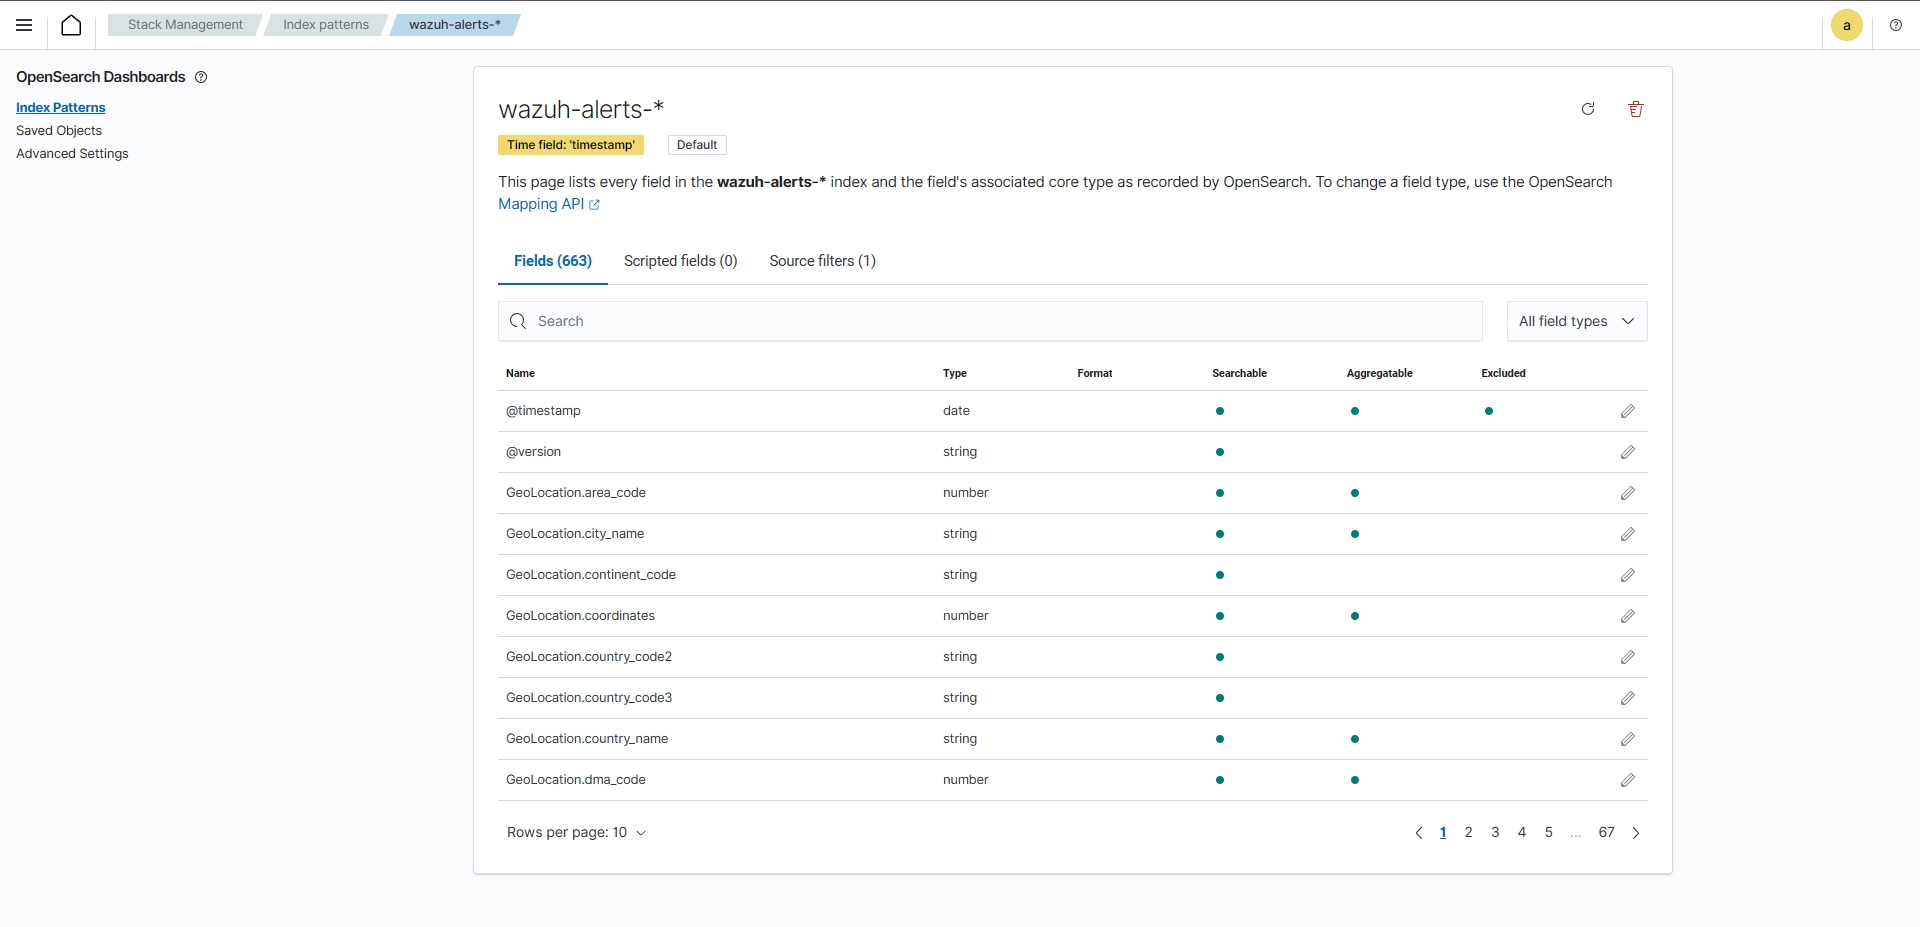
\includegraphics[width=0.8\textwidth]{images/threat-hunting/wazuh-alerts-index-pattern.png}
    \caption{Index patterns on the Wazuh dashboard}
    \label{fig:wazuh-alerts-index-pattern}
\end{figure}

Wazuh's capabilities extend to \textbf{agentless monitoring} and \textbf{syslog data collection}, ensuring efficient log management across various formats. Its indexing and querying features allow for swift data retrieval, aiding in quick analysis and investigations. Advanced parsing and real-time analysis fortify proactive threat identification and mitigation.

\subsubsection{Wazuh Archives}

Wazuh provides a centralized solution for log storage from monitored endpoints, including non-alert generating logs. By default, Wazuh archives are disabled but can be activated easily. Having access to extensive log details is vital for effective threat hunting, offering a comprehensive view of the environment.

\begin{figure}[H]
    \centering
    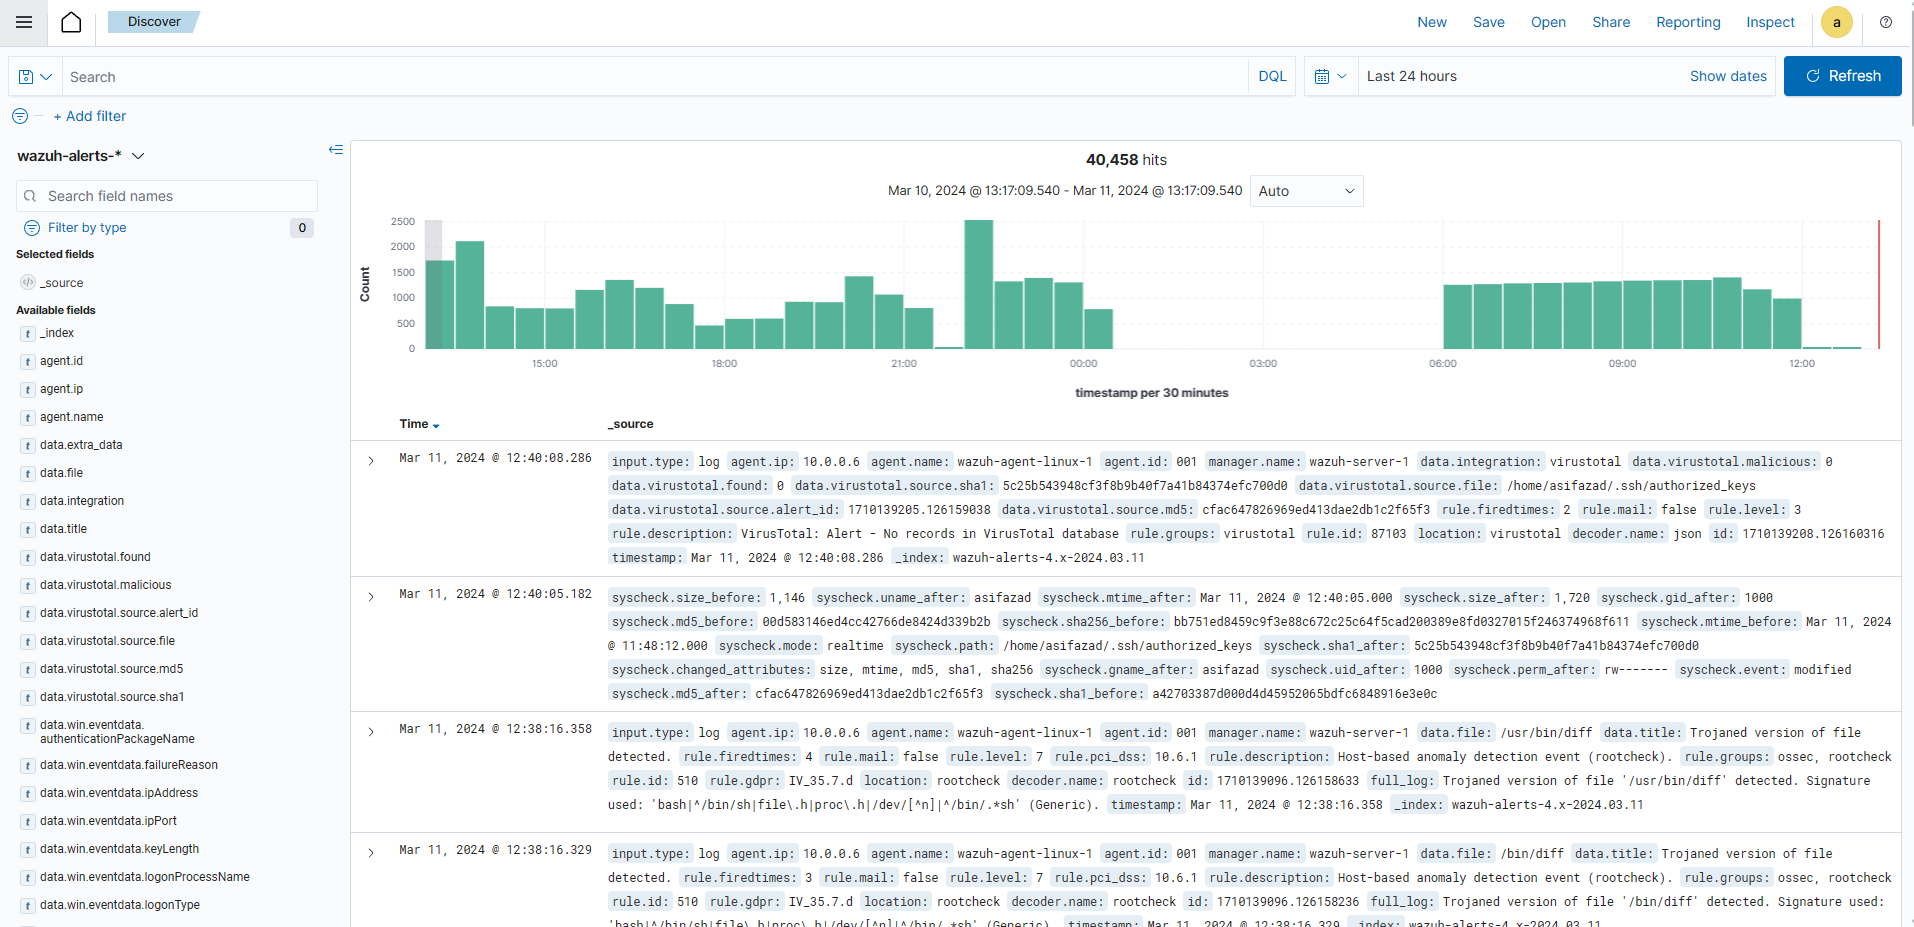
\includegraphics[width=0.8\textwidth]{images/threat-hunting/discover-archives-logs.png}
    \caption{Archived logs in the Discover section of the Wazuh dashboard}
    \label{fig:discover-archives-logs}
\end{figure}

\subsubsection{MITRE ATT\&CK Mapping}

The MITRE ATT\&CK framework provides a structured model to identify and understand cyber attackers' tactics, techniques, and procedures (TTPs). Wazuh's integration with the MITRE ATT\&CK framework aids in identifying TTPs utilized by adversaries, enabling users to defend against them proactively.

For instance, unusual login activities can be associated with specific techniques within the framework, helping in the implementation of countermeasures. We particularly witnessed this because we had a number of agents that had public IP intentionally exposed for SSH connection. We witnessed a flurry of attacks from different corners of the globe, specially from places like Russia, China or North Korea. The Wazuh dashboard offered key insights into these attack techniques and their occurrence within the environment.

\begin{figure}[H]
    \centering
    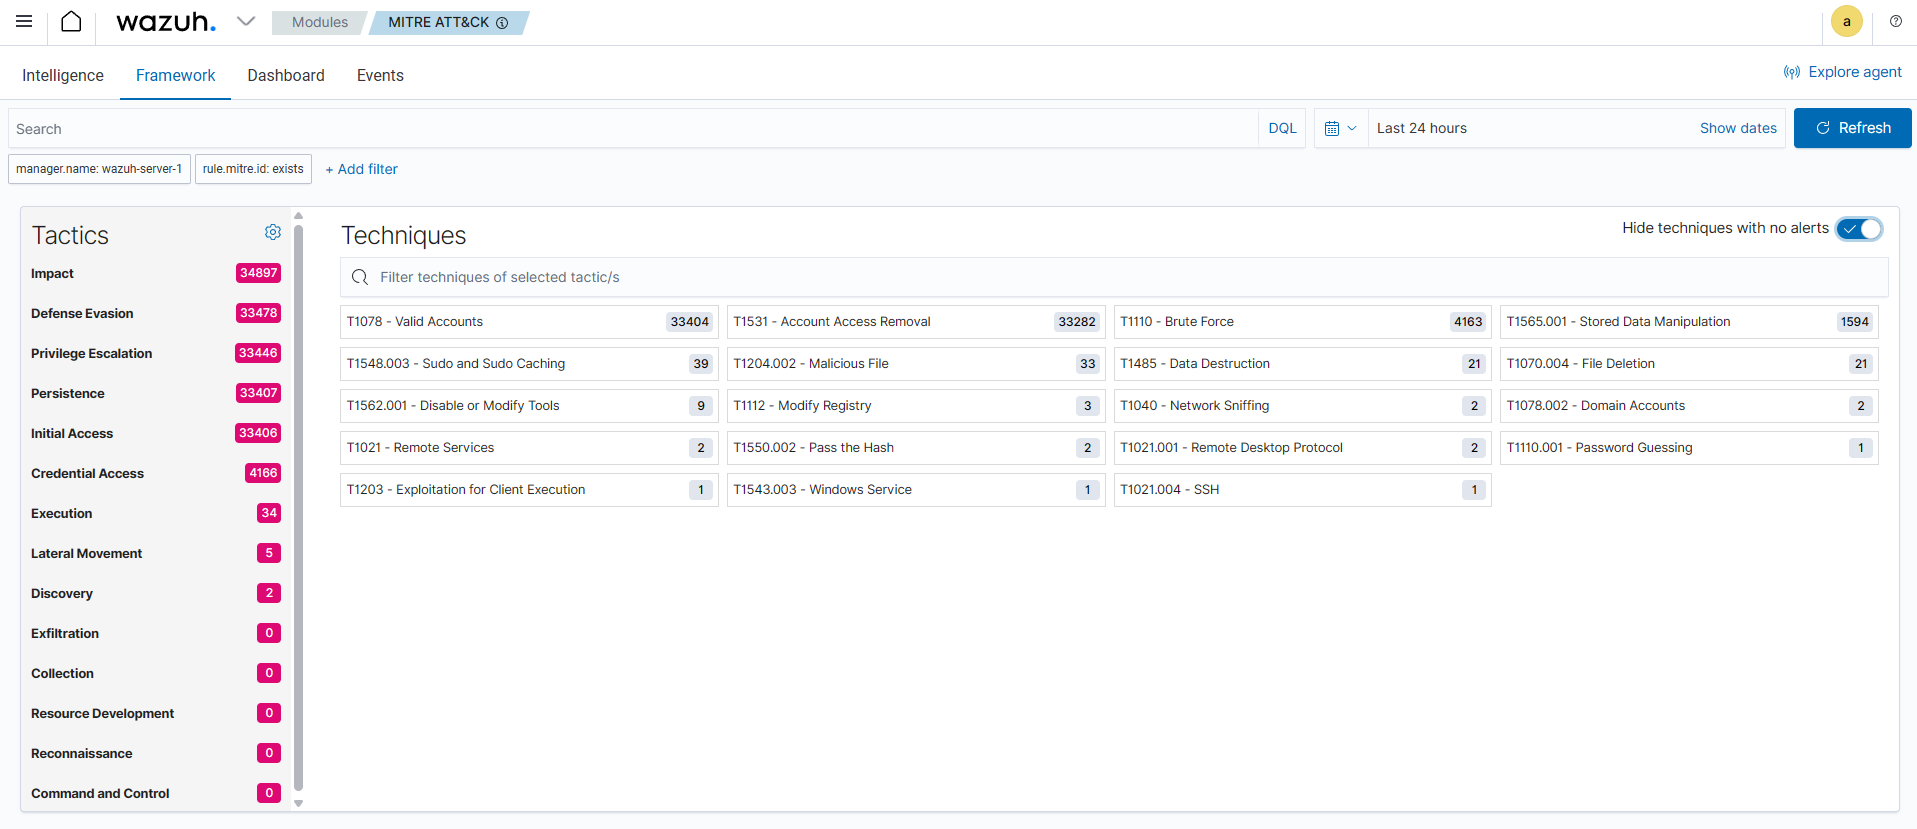
\includegraphics[width=0.7\textwidth]{images/threat-hunting/mitre-techniques.png}
    \caption{MITRE ATT\&CK Module Shows the Common Techniques}
    \label{fig:mitre-attack-techniques}
\end{figure}

The module generates detailed reports and visualizations, highlighting the frequency and severity of specific TTPs, assisting in compliance tracking and security enhancement.

\begin{figure}[H]
    \centering
    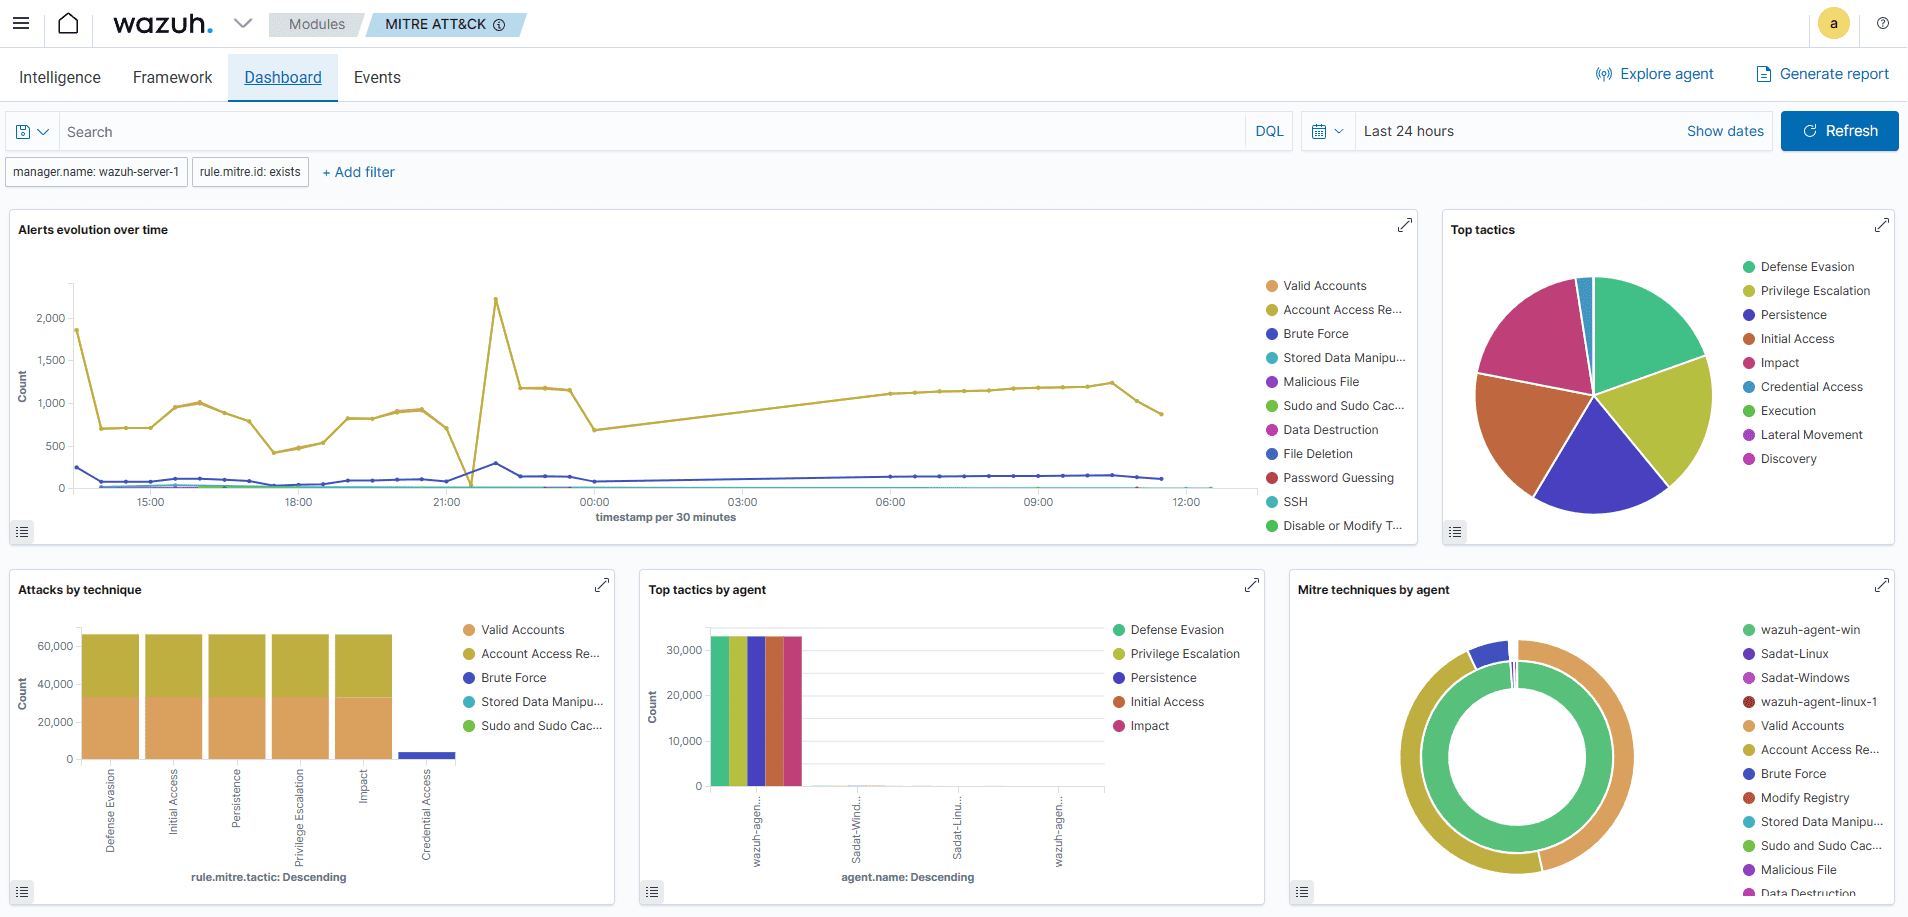
\includegraphics[width=0.8\textwidth]{images/threat-hunting/mitre-dashboard.png}
    \caption{MITRE ATT\&CK module Dashboard on Wazuh}
    \label{fig:mitre-attack-dashboard}
\end{figure}

\subsubsection{Third-party Integration}

Wazuh's compatibility with third-party tools amplifies threat hunting capabilities by consolidating data from diverse sources and automating threat detection and response processes.

Integrations with platforms like VirusTotal (shown in \ref{virustotal}), AlienVault, and MISP, enhance the detection capabilities by allowing cross-referencing of data with threat intelligence feeds.

\subsubsection{Rules and Decoders}

Wazuh's strength in threat hunting is significantly attributed to its comprehensive set of rules, decoders, and pre-configured directives for a multitude of cyber threats and activities.

The management section on the Wazuh dashboard provides insight into both predefined and custom rules applicable to a variety of security incidents.

\begin{figure}[H]
    \centering
    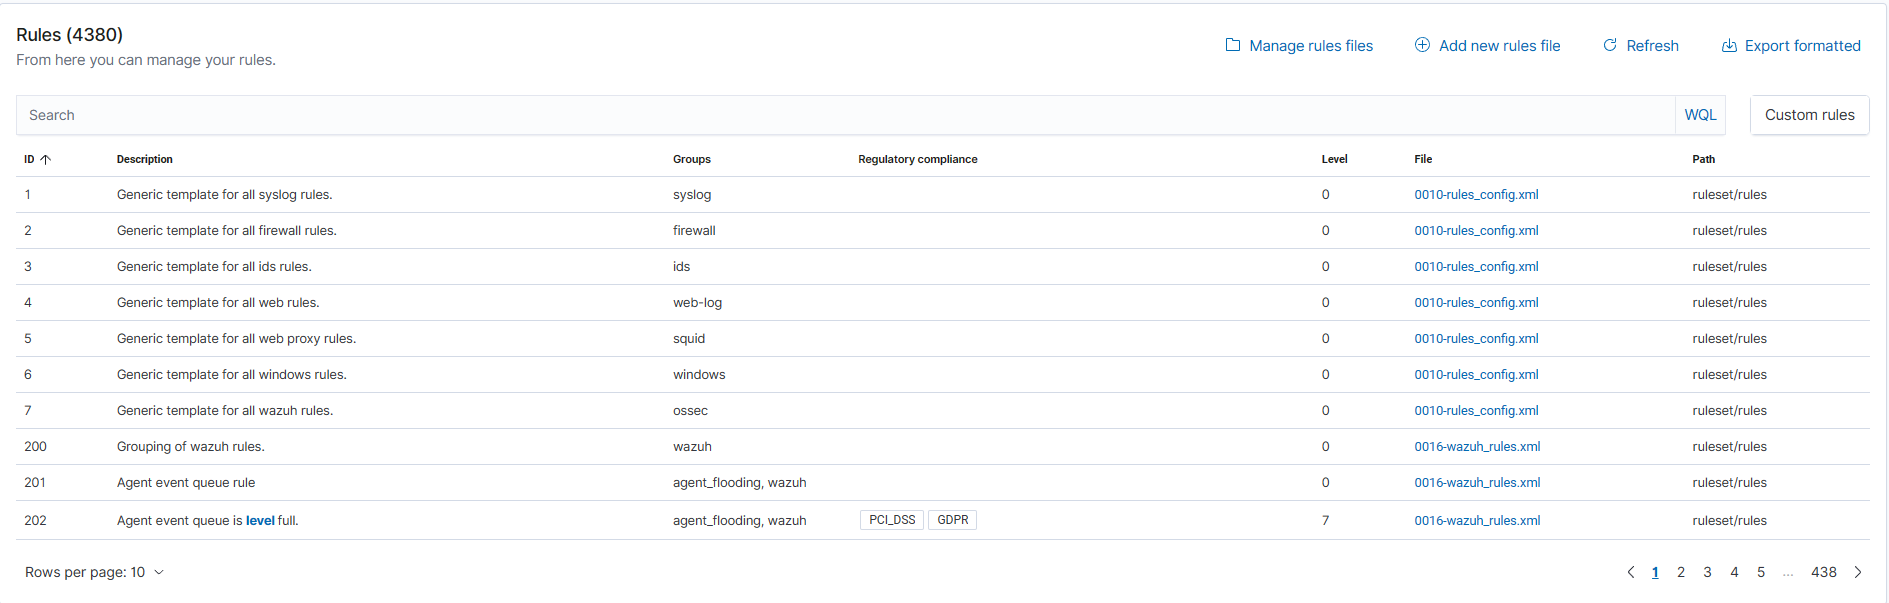
\includegraphics[width=0.8\textwidth]{images/threat-hunting/rules.png}
    \caption{Rules View on the Wazuh Dashboard}
    \label{fig:wazuh-dashboard-rules}
\end{figure}

Decoders play a crucial role in normalizing and interpreting log data, ensuring that information from various sources is standardized for efficient analysis.

\begin{figure}[H]
    \centering
    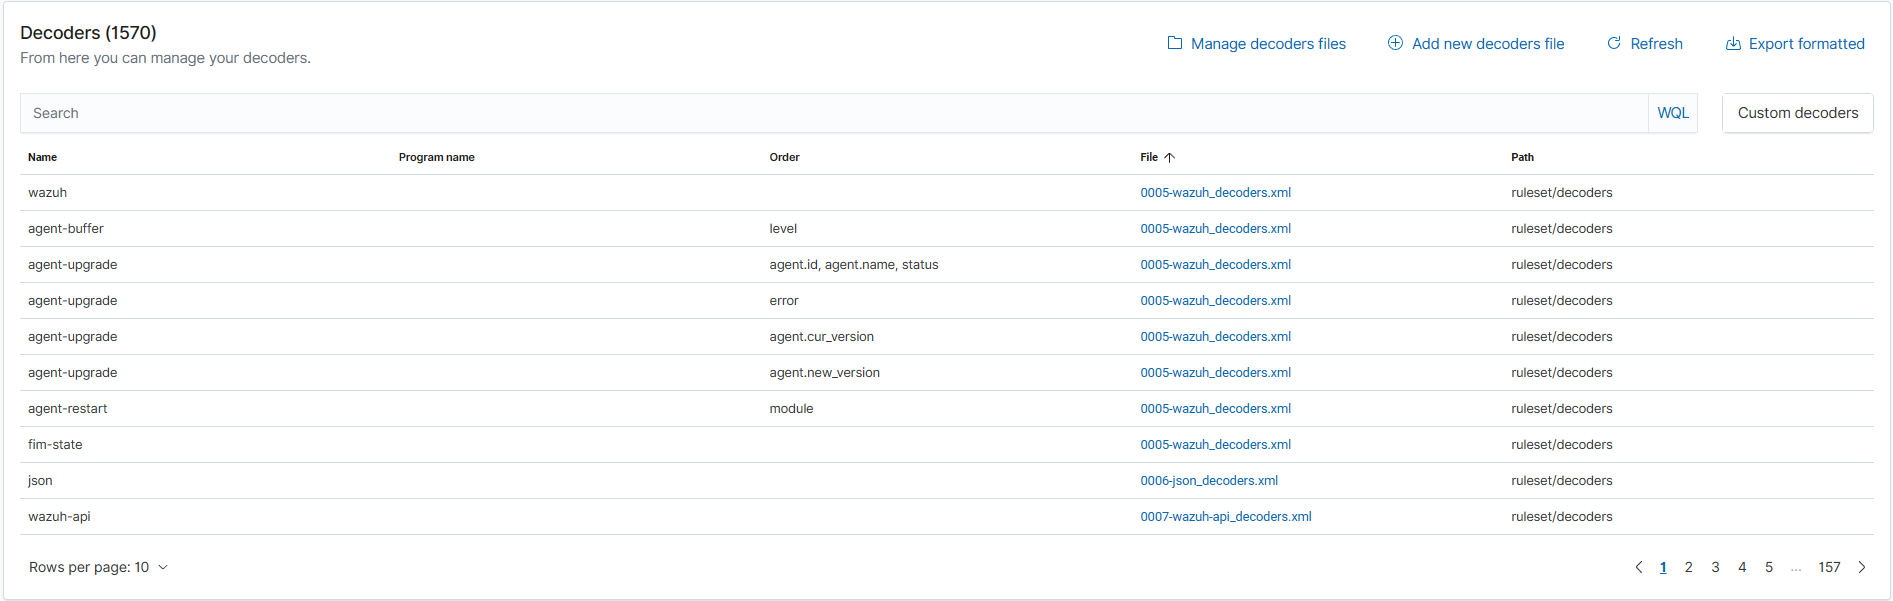
\includegraphics[width=0.8\textwidth]{images/threat-hunting/decoders.png}
    \caption{Decoders View on the Wazuh Dashboard}
    \label{fig:default-decoder-details}
\end{figure}

By leveraging Wazuh's capabilities, security teams gain valuable insights, enabling rapid detection of indicators of compromise, anomalous behavior, and potential security breaches.
